\begin{activity} \label{A:2.2.1}  Consider the function $f(x) = \sin(x)$, which is graphed in Figure~\ref{F:2.2.A1} below.  Note carefully that the grid in the diagram does not have boxes that are $1 \times 1$, but rather approximately $1.57 \times 1$, as the horizontal scale of the grid is $\pi/2$ units per box.
\ba
	\item At each of $x = -2\pi, -\frac{3\pi}{2}, -\pi, -\frac{\pi}{2}, 0, \frac{\pi}{2}, \pi, \frac{3\pi}{2}, 2\pi,$ use a straightedge to sketch an accurate tangent line to $y = f(x)$.
	\item Use the provided grid to estimate the slope of the tangent line you drew at each point.  Pay careful attention to the scale of the grid.
	\item Use the limit definition of the derivative to estimate $f'(0)$ by using small values of $h$, and compare the result to your visual estimate for the slope of the tangent line to $y = f(x)$ at $x = 0$ in (b).  Using periodicity, what does this result suggest about $f'(2\pi)$?  about $f'(-2\pi)$?  
	\item Based on your work in (a), (b), and (c), sketch an accurate graph of $y = f'(x)$ on the axes adjacent to the graph of $y = f(x)$.
	\item What familiar function do you think is the derivative of $f(x) = \sin(x)$?
\ea
\begin{figure}[h]
\begin{center}
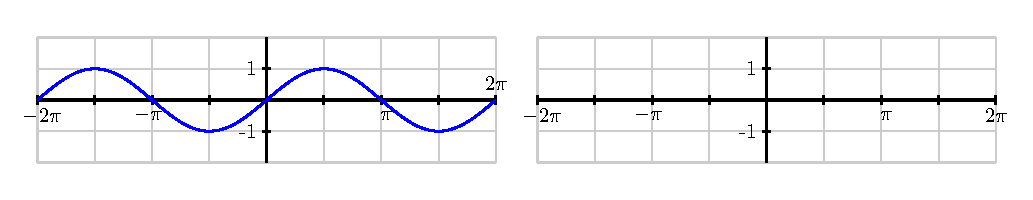
\includegraphics{figures/2_2_sine.eps}
\caption{At left, the graph of $y = f(x) = \sin(x)$.} \label{F:2.2.A1}
\end{center}
\end{figure}

\end{activity}
\begin{smallhint}
\ba
	\item It's very important to use a straightedge for accuracy.
	\item First determine the slopes that appear to be zero.  Then estimate $f'(0)$ carefully using the grid.  Use symmetry and periodicity to help you estimate other nonzero slopes on the graph.
	\item $f'(0) \approx \frac{\sin(h)}{h}$ for small values of $h$. 
	\item Recall that heights on $f'$ come from slopes on $f$.
	\item It might be reasonable to expect that the derivative of a trigonometric function is another trigonometric function.
\ea
\end{smallhint}
\begin{bighint}
\ba
	\item It's very important to use a straightedge for accuracy.
	\item $f'(0) \approx 1$, as for each grid box we move horizontally, we go up about 1.5 grid boxes.
	\item $f'(0) \approx \frac{\sin(h)}{h}$ for small values of $h$.  Try using $h = 0.001$ and $h = -.001$. 
	\item Recall that heights on $f'$ come from slopes on $f$.  From your earlier work, you should know several places $f'(x) = 0$, plus that $f'(0) \approx 1$.  Plot these values on the grid for $y = f'(x)$.
	\item It might be reasonable to expect that the derivative of a trigonometric function is another trigonometric function, or possibly some multiple of such a function.
\ea 
\end{bighint}
\begin{activitySolution}
\ba
	\item See the figure below.
	\item Reading left to right from $-2\pi, \ldots, 2\pi$ with stepsize $\pi/2$, the respective slopes of tangent lines appear to be $1,0,-1,0,1,0,-1,0,1$.
	\item From the limit definition,
	\begin{eqnarray*}
	f'(0) & = & \lim_{h \to 0} \frac{f(0 + h) - f(0)}{h} \\
	       & = & \lim_{h \to 0} \frac{\sin(0 + h) - \sin(0)}{h} \\
	       & = & \lim_{h \to 0} \frac{\sin(h)}{h} 
	\end{eqnarray*}
	Because we cannot simplify the fraction $\frac{\sin(h)}{h}$ any further algebraically, we estimate the value of the limit using small values of $h$.  Doing so, it appears that $\lim_{h \to 0} \frac{\sin(h)}{h}  = 1$, and thus $f'(0) = 1$.  This matches the estimate generated visually by sketching the tangent line at $(0,f(0))$.  Finally, by the periodicity of the sine function, we expect the value of the derivative at 0 to match the derivative value at $-2\pi$ and $2\pi$.
	\item See the figure below.
	\item It appears that $\frac{d}{dx}[\sin(x)] = \cos(x)$.
\ea
%\begin{figure}[h]
\begin{center}
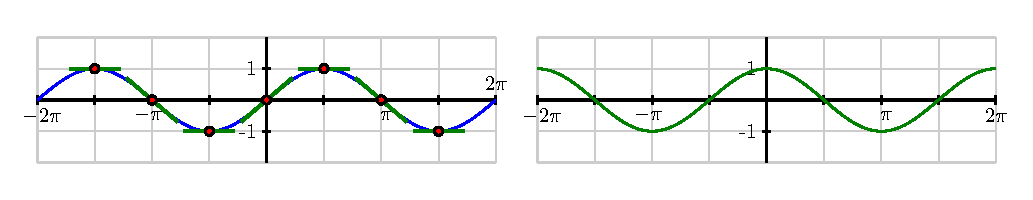
\includegraphics{figures/2_2_sineSoln.eps}
%\caption{At left, the graph of $y = f(x) = \sin(x)$ along with several tangent lines.  At right, the graph of $y = f'(x)$, where the heights on the graph of $f'(x)$ come from slopes on the graph of $f$.} \label{F:2.2.A1Soln}
\end{center}
%\end{figure}
\end{activitySolution}
\aftera